\documentclass[a4paper, 14pt]{extarticle}

% Поля
%--------------------------------------
\usepackage{geometry}
\geometry{a4paper,tmargin=2cm,bmargin=2cm,lmargin=3cm,rmargin=1cm}
%--------------------------------------


%Russian-specific packages
%--------------------------------------
\usepackage[T2A]{fontenc}
\usepackage[utf8]{inputenc} 
\usepackage[english, main=russian]{babel}
%--------------------------------------

\usepackage{textcomp}

% Красная строка
%--------------------------------------
\usepackage{indentfirst}               
%--------------------------------------             


%Graphics
%--------------------------------------
\usepackage{graphicx}
\graphicspath{ {./images/} }
\usepackage{wrapfig}
%--------------------------------------

% Полуторный интервал
%--------------------------------------
\linespread{1.3}                    
%--------------------------------------

%Выравнивание и переносы
%--------------------------------------
% Избавляемся от переполнений
\sloppy
% Запрещаем разрыв страницы после первой строки абзаца
\clubpenalty=10000
% Запрещаем разрыв страницы после последней строки абзаца
\widowpenalty=10000
%--------------------------------------

%Списки
\usepackage{enumitem}

%Подписи
\usepackage{caption} 

%Гиперссылки
\usepackage{hyperref}

\hypersetup {
	unicode=true
}

%Рисунки
%--------------------------------------
\DeclareCaptionLabelSeparator*{emdash}{~--- }
\captionsetup[figure]{labelsep=emdash,font=onehalfspacing,position=bottom}
%--------------------------------------

\usepackage{tempora}

%Листинги
%--------------------------------------
\usepackage{listings}
\lstset{
  basicstyle=\ttfamily\footnotesize, 
  %basicstyle=\footnotesize\AnkaCoder,        % the size of the fonts that are used for the code
  breakatwhitespace=false,         % sets if automatic breaks shoulbd only happen at whitespace
  breaklines=true,                 % sets automatic line breaking
  captionpos=t,                    % sets the caption-position to bottom
  inputencoding=utf8,
  frame=single,                    % adds a frame around the code
  keepspaces=true,                 % keeps spaces in text, useful for keeping indentation of code (possibly needs columns=flexible)
  keywordstyle=\bf,       % keyword style
  numbers=left,                    % where to put the line-numbers; possible values are (none, left, right)
  numbersep=5pt,                   % how far the line-numbers are from the code
  xleftmargin=25pt,
  xrightmargin=25pt,
  showspaces=false,                % show spaces everywhere adding particular underscores; it overrides 'showstringspaces'
  showstringspaces=false,          % underline spaces within strings only
  showtabs=false,                  % show tabs within strings adding particular underscores
  stepnumber=1,                    % the step between two line-numbers. If it's 1, each line will be numbered
  tabsize=2,                       % sets default tabsize to 8 spaces
  title=\lstname                   % show the filename of files included with \lstinputlisting; also try caption instead of title
}
%--------------------------------------

%%% Математические пакеты %%%
%--------------------------------------
\usepackage{amsthm,amsfonts,amsmath,amssymb,amscd}  % Математические дополнения от AMS
\usepackage{mathtools}                              % Добавляет окружение multlined
\usepackage[perpage]{footmisc}
%--------------------------------------

%--------------------------------------
%			НАЧАЛО ДОКУМЕНТА
%--------------------------------------

\begin{document}

%--------------------------------------
%			ТИТУЛЬНЫЙ ЛИСТ
%--------------------------------------
\begin{titlepage}
\thispagestyle{empty}
\newpage


%Шапка титульного листа
%--------------------------------------
\vspace*{-60pt}
\hspace{-65pt}
\begin{minipage}{0.3\textwidth}
\hspace*{-20pt}\centering

\includegraphics[width=\textwidth]{emblem}
\end{minipage}
\begin{minipage}{0.67\textwidth}\small \textbf{
\vspace*{-0.7ex}
\hspace*{-6pt}\centerline{Министерство науки и высшего образования Российской Федерации}
\vspace*{-0.7ex}
\centerline{Федеральное государственное бюджетное образовательное учреждение }
\vspace*{-0.7ex}
\centerline{высшего образования}
\vspace*{-0.7ex}
\centerline{<<Московский государственный технический университет}
\vspace*{-0.7ex}
\centerline{имени Н.Э. Баумана}
\vspace*{-0.7ex}
\centerline{(национальный исследовательский университет)>>}
\vspace*{-0.7ex}
\centerline{(МГТУ им. Н.Э. Баумана)}}
\end{minipage}
%--------------------------------------

%Полосы
%--------------------------------------
\vspace{-25pt}
\hspace{-35pt}\rule{\textwidth}{2.3pt}

\vspace*{-20.3pt}
\hspace{-35pt}\rule{\textwidth}{0.4pt}
%--------------------------------------

\vspace{1.5ex}
\hspace{-35pt} \noindent \small ФАКУЛЬТЕТ\hspace{80pt} <<Информатика и системы управления>>

\vspace*{-16pt}
\hspace{47pt}\rule{0.83\textwidth}{0.4pt}

\vspace{0.5ex}
\hspace{-35pt} \noindent \small КАФЕДРА\hspace{50pt} <<Теоретическая информатика и компьютерные технологии>>

\vspace*{-16pt}
\hspace{30pt}\rule{0.866\textwidth}{0.4pt}
  
\vspace{11em}

\begin{center}
\Large {\bf Лабораторная работа № 4} \\ 
\large {\bf по курсу <<Компьютерные сети>>} \\
\large <<SSH>> 
\end{center}\normalsize

\vspace{8em}


\begin{flushright}
  {Студент группы ИУ9-32Б Волохов А. В. \hspace*{15pt}\\ 
  \vspace{2ex}
  Преподаватель Посевин Д. П.\hspace*{15pt}}
\end{flushright}

\bigskip

\vfill
 

\begin{center}
\textsl{Москва 2023}
\end{center}
\end{titlepage}
%--------------------------------------
%		КОНЕЦ ТИТУЛЬНОГО ЛИСТА
%--------------------------------------

\renewcommand{\ttdefault}{pcr}

\setlength{\tabcolsep}{3pt}
\newpage
\setcounter{page}{2}
\section{Задание}\label{Sect::task}
Рассматривается задача разработки SSH-сервера на языке GO
Рассматривается задача разработки SSH-клиента на языке GO


Исходный код программы представлен в листингах~\ref{lst:code1}--~\ref{lst:code2}--~\ref{lst:code3}--~\ref{lst:code4}--~\ref{lst:code5}--~\ref{lst:code6}.

\begin{figure}[!htb]
\begin{lstlisting}[language={Go},caption={client.go},label={lst:code1}]
package main

import (
	"bufio"
	"fmt"
	"golang.org/x/crypto/ssh"
	"os"
	"strings"
)

func main() {
	reader := bufio.NewReader(os.Stdin)

	fmt.Print("SSH Server Address: ")
	serverAddress, _ := reader.ReadString('\n')
	serverAddress = strings.TrimSpace(serverAddress)

	fmt.Print("Username: ")
	username, _ := reader.ReadString('\n')
	username = strings.TrimSpace(username)

	fmt.Print("Password: ")
	password, _ := reader.ReadString('\n')
	password = strings.TrimSpace(password)

	config := &ssh.ClientConfig{
		User: username,
		Auth: []ssh.AuthMethod{
			ssh.Password(password),
		},
		HostKeyCallback: ssh.InsecureIgnoreHostKey(),
	}

	client, err := ssh.Dial("tcp", serverAddress, config)
	if err != nil {
		fmt.Println("Failed to connect to the SSH server:", err)
		return
	}
	defer func(client *ssh.Client) {
		err := client.Close()
		if err != nil {

		}
	}(client)
	currentDir := "" // Текущая директория

	for {
		fmt.Print("Enter SSH command (or 'exit' to quit): ")
		command, _ := reader.ReadString('\n')
		command = strings.TrimSpace(command)

		if command == "exit" {
			break
		}
		session, err := client.NewSession()
		if err != nil {
			fmt.Println("Failed to create SSH session:", err)
			continue
		}

\end{lstlisting}
\end{figure}

\newpage

\begin{figure}[!htb]
\begin{lstlisting}[language={Go},caption={client.go - продолжение},label={lst:code2}]
switch {
		case strings.HasPrefix(command, "ls"):
			output, err := session.CombinedOutput("ls " + currentDir)
			err = session.Close()
			if err != nil {return}
			if err != nil {fmt.Println("Failed to list directory:", err)}
                else {fmt.Println("Directory contents:\n", string(output))}
		case strings.HasPrefix(command, "cd"):
			newDir := strings.TrimSpace(strings.TrimPrefix(command, "cd"))
			Path := newDir
			if currentDir != "" {Path = currentDir + "/" + newDir}
			output, err := session.CombinedOutput("cd " + Path + " && pwd")
			currentDir = Path
			err = session.Close()
			if err != nil {
				return
			}
			if err != nil {
				fmt.Println("Failed to change directory:", err)
			} else {
				currentDir = strings.TrimSpace(string(output))
				fmt.Println("Current directory:", currentDir)
			}
		case strings.HasPrefix(command, "mkdir"):
			dirName := strings.TrimSpace(strings.TrimPrefix(command, "mkdir"))
			_, err := session.CombinedOutput("mkdir " + currentDir + "/" + dirName)
			if err != nil {
				fmt.Println("Failed to create directory:", err)
			} else {
				fmt.Println("Directory created:", dirName)
			}
		case strings.HasPrefix(command, "rmdir"):
			dirName := strings.TrimSpace(strings.TrimPrefix(command, "rmdir"))
			Path := dirName
			if currentDir != "" {
				Path = currentDir + "/" + dirName
			}
			_, err := session.CombinedOutput("rmdir " + Path)
			if err != nil {
				fmt.Println("Failed to remove directory:", err)
			} else {
				fmt.Println("Directory removed:", dirName)
			}
		case strings.HasPrefix(command, "mv"):
			args := strings.Split(command, " ")
			if len(args) != 3 {
				fmt.Println("Usage: mv source destination")
			} else {
				sourcePath := args[1]
				destPath := args[2]
				_, err := session.CombinedOutput("mv " + sourcePath + " " + destPath)
				if err != nil {
					fmt.Println("Failed to move:", err)
				} else {
					fmt.Println("Moved:", sourcePath, "to", destPath)
				}}

\end{lstlisting}
\end{figure}

\newpage
\begin{figure}[!htb]
\begin{lstlisting}[language={Go},caption={client.go - продолжение},label={lst:code3}]
default:
			output, err := session.CombinedOutput(command)

			if err != nil {
				fmt.Println("Failed to execute the command:", err)
			} else {
				fmt.Println("Command output:\n", string(output))
			}
		}
	}

	fmt.Println("SSH session ended.")
}
\end{lstlisting}
\end{figure}
\newpage
\begin{figure}[!htb]
\begin{lstlisting}[language={Go},caption={server.go},label={lst:code4}]
package main

import (
	"fmt"
	"github.com/gliderlabs/ssh"
	"golang.org/x/crypto/ssh/terminal"
	"io"
	"log"
	"os"
	"os/exec"
	"strings"
)

var path = "./lab4/server/server_space/"
var authorizedKeysPath = "./lab4/server/authorized_keys"

func handleSession(session ssh.Session) {
	term := terminal.NewTerminal(session, "enter command >> ")
	io.WriteString(session, fmt.Sprintf("Successful login, %s\n", session.User()))
	for {
		command, err := term.ReadLine()
		if err != nil {
			log.Println(err)
		}
		log.Printf("Received %s: %s", session.User(), command)
		selectCommand(session, command)
	}
}

func selectCommand(session ssh.Session, command string) {
	switch command {
	case "exit":
		return
	case "ping":
		output, err := runCommand("ping", "-c", "4", "google.com")
		if err != nil {
			io.WriteString(session, fmt.Sprintf("Error ping: %s\n", err))
		} else {
			io.WriteString(session, string(output))
		}
	default:
		args := strings.Fields(command)
		if len(args) > 0 {
			switch args[0] {

			case "mkdir":
				if len(args) < 2 {
					io.WriteString(session, "You must specify dir name\n")
				} else {
					err := os.Mkdir(path+args[1], 0755)
					if err != nil {
						io.WriteString(session, fmt.Sprintf("Failed to create dir: %s\n", err))
					} else {
						io.WriteString(session, "Dir created\n")
					}
				}

\end{lstlisting}
\end{figure}
\newpage
\begin{figure}[!htb]
\begin{lstlisting}[language={Go},caption={server.go - продолжение},label={lst:code5}]
case "rmdir":
				if len(args) < 2 {
					io.WriteString(session, "You need to specify dir to delete\n")
				} else {
					err := os.Remove(path + args[1])
					if err != nil {
						io.WriteString(session, fmt.Sprintf("Failed to delete: %s\n", err))
					} else {
						io.WriteString(session, "Dir successfully deleted\n")
					}
				}

			case "ls":
				files, err := os.ReadDir(path)
				if err != nil {
					io.WriteString(session, fmt.Sprintf("Error reading dir: %s\n", err))
				} else {
					var output strings.Builder
					for _, file := range files {
						output.WriteString(file.Name())
						output.WriteString("\n")
					}
					io.WriteString(session, output.String())
				}

			case "mv":
				if len(args) < 3 {
					io.WriteString(session, "You need to specify src and dst paths\n")
				} else {
					err := os.Rename(path+args[1], path+args[2]+"/"+args[1])
					if err != nil {
						io.WriteString(session, fmt.Sprintf("Error while moving: %s\n", err))
					} else {
						io.WriteString(session, "File successfully moved\n")
					}
				}

			case "rm":
				if len(args) < 2 {
					io.WriteString(session, "You need to specify file to delete\n")
				} else {
					err := os.Remove(path + args[1])
					if err != nil {
						io.WriteString(session, fmt.Sprintf("Error while deleting: %s\n", err))
					} else {
						io.WriteString(session, "Successfully deleted\n")
					}
				}
			case "cd":
				if len(args) < 2 {
					io.WriteString(session, "You need to specify dir to change\n")
				} else {
					_, err := os.ReadDir(path + args[1])
\end{lstlisting}
\end{figure}

\newpage

\begin{figure}[!htb]
\begin{lstlisting}[language={Go},caption={server.go - продолжение},label={lst:code6}]
if err != nil {
						io.WriteString(session, fmt.Sprintf("Error - no such dir: %s\n", err))
					} else {
						io.WriteString(session, "Dir changed successfully\n")
						path += args[1] + "/"
					}
				}

			default:
				io.WriteString(session, "Wrong command\n")
			}
		} else {
			io.WriteString(session, "Wrong command\n")
		}
	}
}

func runCommand(name string, args ...string) ([]byte, error) {
	cmd := exec.Command(name, args...)
	output, err := cmd.CombinedOutput()

	if err != nil {
		return nil, fmt.Errorf("command execution failed with: %s", err)
	}
	return output, nil
}

func main() {
	server := ssh.Server{
		Addr: "localhost:2222",
		Handler: func(s ssh.Session) {
			handleSession(s)
		},
		PasswordHandler: func(ctx ssh.Context, password string) bool {
			log.Printf("User authentication %s", ctx.User())
			return true
		},
	}
	log.Println("SSH started at port 2222")

	err := server.ListenAndServe()
	if err != nil {
		log.Fatalf("Error starting server: %v", err)
	}
}

\end{lstlisting}
\end{figure}

\newpage

\begin{figure}[!htb]
	\centering
	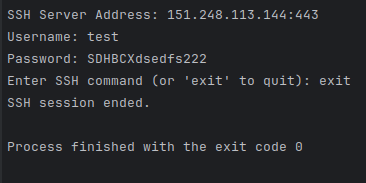
\includegraphics[width=0.8\textwidth]{res1.png}
\caption{Клиент}
\label{fig:img1}
\end{figure}
\begin{figure}[!htb]
	\centering
	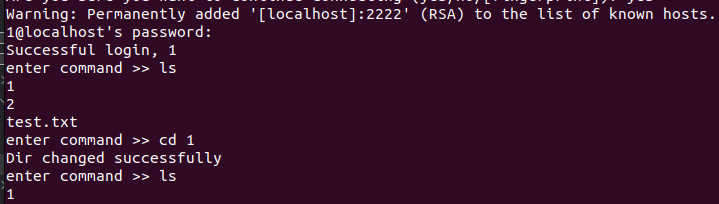
\includegraphics[width=0.8\textwidth]{res2.png}
\caption{Сервер}
\label{fig:img2}
\end{figure}





\end{document}
